\documentclass[hidelinks,12pt]{article}

\usepackage{amsmath}    % need for subequations
\usepackage{graphicx}   % need for figures
\usepackage{verbatim}   % useful for program listings
\usepackage{color}      % use if color is used in text
\usepackage{subfigure}  % use for side-by-side figures
\usepackage{hyperref}   % use for hypertext links, including those to external documents and URLs

\usepackage[numbered]{matlab-prettifier} % including matlab w/ syntax highlighting
\usepackage[T1]{fontenc} % prettier matlab font
\lstMakeShortInline[style=Matlab-editor]| % matlab inline escape character

\usepackage[
top    = 2.75cm,
bottom = 2.50cm,
left   = 3.00cm,
right  = 2.50cm]{geometry}

\graphicspath{ {./Figures/} }

% don't need the following. simply use defaults
\setlength{\baselineskip}{16.0pt}    % 16 pt usual spacing between lines



\begin{document}
\pagenumbering{gobble}
\begin{center}
  {\huge Homework 5}\\
  \vspace{10px}
  
\includegraphics{Logo} \\
  Date of Submission:\\
  February 25, 2019\\
  \vspace{30px}
  \rule{300px}{0.5px} \\
  Thorne Wolfenbarger \\
  \href{mailto:wolfent1@my.erau.edu}{wolfent1@my.erau.edu} \\
  \vspace{30px}
  Submitted to: \\
  Professor Kaela Martin \\
  College of Engineering \\
  \vspace{40px}
  In Partial Fulfillment \\
  of the Requirements of \\
  \vspace{10px}
  AE 313 \\
  Space Mechanics \\
  Spring, 2019 \\
\end{center}

\pagenumbering{arabic}
\begin{center}
\large AE 313 Homework 10
\end{center}
\flushleft
1. Find the minimum $\Delta v_{Total}$ over the range of departure true anomolies.\\
~$\Delta v_{min}=2.6027~km/s$\\

\vspace{10px}
2. Find the corresponding $a_t, e_t, \theta^{^*}_D, v_A, v_D, \gamma_A, \gamma_D$.\\
\begin{tabular}{llll}
$a_t=$&19032~km&$e_t=$&0.4473\\
$\theta^{^*}_D=$&$25.3460^\circ$\\
$v_A=$&$2.9599~km/s$&$v_D=$&$7.2513~km/s$\\
$\gamma_A=$&$11.2794$&$\gamma_D=$&$7.7643^\circ$
\end{tabular}

\vspace{10px}
3. Plot the true anomoly at departure vs the flight path angle. Mark minimum $\Delta v$. Why is the minimum $\Delta v$ when the flight path angles are small?\\
\begin{figure}[!htb]
  \center
  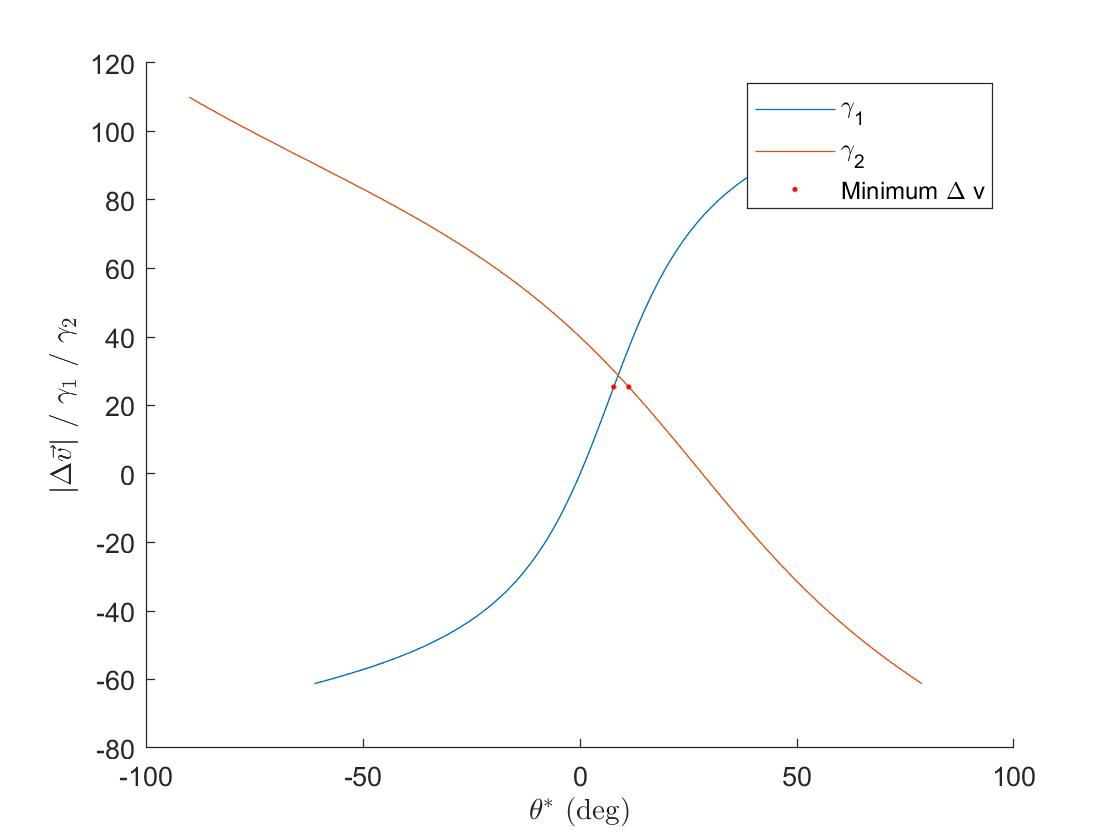
\includegraphics[scale=0.4]{FPAGraphs}
  \caption{$\theta^{^*}_D~vs.~\gamma_D~\&~\gamma_A$}
  \label{fig:ta-vs-fpa}
\end{figure}
The minimum $\Delta v$ occurs when the flight path angles are low because the maneuver to change the angle of flight is expensive whereas an in-line velocity change is cheap. The low flight path angles indicate that most of the change in velocity is in-line; implying a cheap total transfer.


\vspace{10px}
4. What type of transfer is the minimal $\Delta v$ transfer?\\
~The minimal $\Delta v$ transfer orbit is a 1A Elliptical Transfer.\\


\vspace{10px}
5. Plot the two circular orbits and the transfer orbit. Mark the following quantities: $\vec{r}_D, \vec{v}_D, \gamma_D, \Delta \vec{v}_D, \alpha_D, \vec{r}_A, \vec{v}_A, \gamma_A, \Delta \vec{v}_A, \alpha_A$.\\
\begin{figure}[!htb]
  \center
  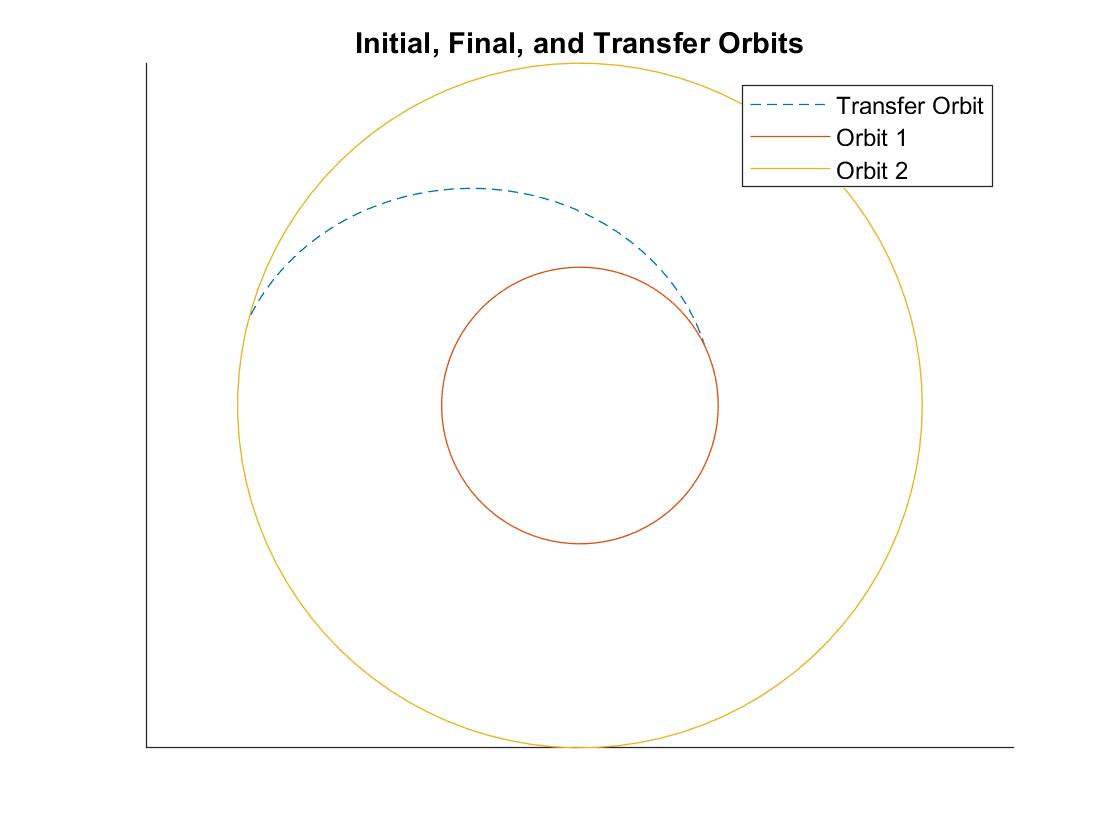
\includegraphics[scale=0.4]{orbits}
  \caption{Infinite Diagram}
  \label{fig:Fig02}
\end{figure}

\vspace{10px}
6. How does the transfer compare to the minimum energy transfer?\\
The minimum delta v transfer orbit saves $1.0173~km/s$ of delta v compared
to the minimum energy orbit. The semi-major axis of the min-dv transfer
orbit is larget than the semi-major axis of the minimum energy orbit.
This indicated that the minimum $\Delta v$ transfer will have a longer TOF.\\
\newpage
HW5.m
\begin{lstlisting}[frame=lines,style=Matlab-editor,basicstyle = \mlttfamily]
clc; clear all; close all

%constants
MU = 42828;

% Problem 1
vr = [-2089.6 -2515.7 -6382.0];
vv = [2.1744 0.76911 0.13452];

r = norm(vr)
v = norm(vv)

vh = cross(vr, vv);
h = norm(vh);

syms a
energy_eqn = v^2/2 - MU/r == -MU/(2*a)
energy = v^2/2 - MU/r
a = double(solve(energy_eqn, a))

syms e
h_eqn = h == sqrt(MU*a*(1-e^2))
e = double(solve(h_eqn,e))
e = max(e)

syms E
E_eqn = r == a*(1-e*cos(E));
E = double(solve(E_eqn,E));
E = -min(E) %Because it is descending.

syms time_since_p
time_since_p_eqn = sqrt(MU/a^3)*time_since_p == E - e*sin(E);
time_since_p = double(solve(time_since_p_eqn,time_since_p))

% Problem 2
p = h^2/MU;
true_a = -acos(p/(r*e) - 1/e)
vv_rt = [h*e/p*sin(true_a) h/r 0] % answer

% Problem 3
E1 = E;
t1 = time_since_p;
vr1 = vr;
vv1 = vv;
r1 = r;
v1 = v;
t2 = time_since_p + 12*60*60;
n = sqrt(MU/a^3);
M = n*t2;
E2 = fzero(@(x) x-e*sin(x)-M, 0);
f = 1 - a/r*(1-cos(E2-E1));
g = (t2 - t1) - sqrt(a^3/MU)*(E2 - E1 - sin(E2 - E1));

vr2 = f*vr + g*vv;
r2 = norm(vr2);
fdot = -sqrt(MU*a)/(r2*r1)*sin(E2-E1);
gdot = 1 - a/r2*(1-cos(E2-E1));

vv2 = fdot*vr1 + gdot*vv1 % intertial unit vectors

true_a2 = -acos(p/(r2*e) - 1/e)

vv2_rt = [h*e/p*sin(true_a2) h/r2 0] % radial-tangential

% Problem 4
vr2_peri = [r2*cos(true_a2) r2*sin(true_a2) 0]
vv2_peri = sqrt(MU/p)*[-sin(true_a2) e+cos(true_a2) 0]

% Problem 5

% find i theta omega
syms inc
h_hat = cross(vr2, vv2)/norm(cross(vr2, vv2))
inc_eqn = cos(inc) == dot(h_hat, [0 0 1])
inc = double(solve(inc_eqn,inc))
inc = max(inc)

syms RAAN
RAAN_eqn_1 = sin(RAAN)*sin(inc) == dot(h_hat, [1 0 0])
RAAN_eqn_2 = -cos(RAAN)*sin(inc) == dot(h_hat, [0 1 0])
RAAN1 = double(solve(RAAN_eqn_1));
RAAN2 = double(solve(RAAN_eqn_2));
RAAN = min(RAAN1)*180/pi

syms arg_peri
r1_hat = vr1/norm(vr1)
theta_hat = cross(r1_hat, h_hat)/norm(cross(r1_hat, h_hat))
syms theta
theta_eqn_1 = sin(inc) * sin(theta) == dot(r1_hat, [0 0 1])
theta_eqn_2 = sin(inc) * cos(theta) == dot(theta_hat, [0 0 1])
theta1 = double(solve(theta_eqn_1, theta))
theta2 = double(solve(theta_eqn_2, theta))
theta = intersect(theta1, theta2)
arg_peri_eqn = arg_peri == theta - true_a
arg_peri = double(solve(arg_peri_eqn, arg_peri))
\end{lstlisting}

\end{document}
